\chapter{Methods}
\label{ch:methods}
We provide the foundation for quantitative conflict analysis of objective functions in multi-objective systems. The analysis centers on the use of three conflict metrics: two existing measures from EMO and one that we have developed and introduce for the first time here. Two case studies on competing objectives in forest management serve to illustrate this conflict analysis. Prior to describing the case studies, we first define terminology and describe each of the measures used.

\section{Terminology}
\label{sec:terminology}
  
\paragraph{The multi-objective problem}
Consider the $M$-objective optimization problem
\begin{align}
\text{Maximize}& \notag \\
& \mathbf{f} = [f_1(\mathbf{x}), f_2(\mathbf{x}), \ldots, f_M(\mathbf{x}) ] \label{eqn:generalObj}\\
\text{subject to}& \notag \\
& \mathbf{x} \in X \label{eqn:generalConstraint}
\end{align}
with \textit{objective functions} $f_i(\mathbf{x}), i \in \{1,\ldots,M\}$ and feasible \textit{decision vectors} (or \textit{solutions}) $\mathbf{x} \in \mathbb{R}^n$ where $n$ is the number of decision variables in the optimization problem. A set of equality and inequality constraints determine the \textit{feasible decision space} $X$. Solutions in $X$ are referenced by superscripts: $X = \{\mathbf{x}^1,\mathbf{x}^2,\ldots,\mathbf{x}^{|X|}\}$. Each objective function $f_i : \mathbb{R}^n \mapsto \mathbb{R}$ maps decision vectors to scalars in $\mathbb{R}$. The vector objective function $\mathbf{f} : X \mapsto \mathbb{R}^M$ maps the feasible decision space to the \textit{objective space} $\mathbb{R}^M$. The set of all objective functions is the \textit{objective set} $\mathcal{M} = \{f_1,\ldots,f_M\}$.

\paragraph{Dominance and frontiers}
A solution $\mathbf{x}^1$ is said to \textit{dominate} another solution $\mathbf{x}^2$ ($\mathbf{x}^1 \succ \mathbf{x}^2$) if
\begin{align}
\exists f_i \in \mathcal{M} : f_i(\mathbf{x}^1) > f_i(\mathbf{x}^2) \text{ and } \forall f_i \in \mathcal{M} \; f_i(\mathbf{x}^1) \ge f_i(\mathbf{x}^2)
\end{align}
A solution $\mathbf{x}^1 \in X$ is \textit{non-dominated} if
\begin{align}
\nexists \mathbf{x}^2 \in X : \mathbf{x}^2 \succ \mathbf{x}^1
\end{align}
For a rational decision maker, all dominated solutions may be removed from the analysis, since for a dominated solution $\mathbf{x}^2$ there exists another solution $\mathbf{x}^1$ which is better: $\mathbf{x}^1$ achieves more in at least one objective than $\mathbf{x}^2$, and $\mathbf{x}^1$ does not achieve less in any objective than $\mathbf{x}^2$. Thus, the decision maker will always select a solution from the set of non-dominated decision vectors that solve the multi-objective problem \eqref{eqn:generalObj} and \eqref{eqn:generalConstraint}. We refer to this set as the \textit{Pareto-optimal set} $P = \{\mathbf{x} \in X | \nexists \mathbf{y} \in X : \mathbf{y} \succ \mathbf{x} \}$.

The \textit{Pareto-optimal frontier}, the \textit{efficient frontier} or, simply, the \textit{frontier} $Z$ is the corresponding set of $M$-dimensional \textit{objective vectors} $\mathbf{z} = [f_1(\mathbf{x}),f_2(\mathbf{x}),\ldots,f_M(\mathbf{x})]$. That is,
\begin{align}
Z = \{\mathbf{z} = [f_1(\mathbf{x}),\ldots,f_M(\mathbf{x})] \:|\: \mathbf{x} \in P\}
\end{align}
We say that a frontier $Z_1$ dominates another frontier $Z_2$ $Z_1 \succ Z_2$ if for each $\mathbf{z}^2 \in Z_2$,
\begin{align}
\exists \mathbf{z}^1 \in Z_1 : \mathbf{z}^1 \succ \mathbf{z}^2.
\end{align}

Objective vectors provide the decision maker with knowledge of the objective achievement of a solution $\mathbf{x}$ -- the $i$th component of an objective vector $\mathbf{z}$ represents the achievement in objective $i$ by the corresponding decision vector $\mathbf{x}$. Objective vectors' components are referred to using subscripts:
\begin{align}
\mathbf{z} = [z_1, z_2, \ldots, z_M]
\end{align}

\paragraph{Ideal and nadir objective vectors}
The \textit{ideal objective vector} is defined as the vector
\begin{align}
\mathbf{z}^{\text{ideal}} = \max_{\mathbf{x} \in X}\{f_i(\mathbf{x})\} \quad \forall i \in \mathcal{M}.
\end{align}
Analogously, define the nadir solution as the vector
\begin{align}
\mathbf{z}^{\text{nadir}} = \min_{\mathbf{x} \in X}\{f_i(\mathbf{x})\} \quad \forall i \in \mathcal{M}.
\end{align}
The ideal objective vector represents the impossible ideal scenario in which each objective is simultaneously optimized. The nadir objective vector represents the worst case scenario in which each objective attains its lowest value. These solutions are the diagonal corners of the minimum bounding box for the efficient frontier $Z$. Since together they provide upper and lower bounds for each objective, they serve as reference points against which the decision maker can compare solutions. 

\paragraph{Trade-offs}
The \textit{trade-off} between two objective vectors $\mathbf{z}^1$ and $\mathbf{z}^2$ is the vector of differences in their objective achievements:
\begin{align}
\mathbf{\tau}^{1,2} = [z^2_1 - z^1_1, z^2_2 - z^1_2, \ldots, z^2_M - z^1_M]
\end{align}
The components of $\mathbf{\tau}^{1,2}$ represent the amount of each objective that would be sacrificed or gained if the decision maker selected solution $\mathbf{z}^2$ instead of $\mathbf{z}^1$.
Note that $\mathbf{\tau}^{1,2} = - \mathbf{\tau}^{2,1}$. 

\paragraph{Sub-dimensions}
During analysis, we often wish to consider only a subset of the objectives $\mathcal{L} \subset\mathcal{M}$. We define such subsets as \textit{sub-dimensional objective sets}. In these cases, it is simpler to work with constructs that have only those components that correspond to the objectives in $\mathcal{L}$. For instance, define the \textit{sub-dimensional objective vector} for the solution $\mathbf{x}^i$ as $\mathbf{z}^i_\mathcal{L}$ which has components $\forall \ell \in \mathcal{L} \; z^i_\ell = f_\ell(\mathbf{x}^i)$.
Define the \textit{sub-dimensional trade-off} $\tau^{1,2}_\mathcal{L}$ as the vector with components $\forall \ell \in \mathcal{L} \; \tau^{1,2}_\ell$.

\paragraph{Relative objective achievements, relative objective vectors, and relative trade-offs}
Using the nadir and ideal objective vectors, we can represent each solution as a vector of its relative objective achievements, each taking a value in $[0,1]$. This allows for dimensionless and scale-agnostic comparison of solutions. For an objective vector $\mathbf{z}$, its \textit{relative achievement in objective} $i$ is
\begin{align}
\overbar{z_i} = \frac{z_i - z^\text{nadir}_i}{z^\text{ideal}_i - z^\text{nadir}_i},
\end{align}
and the corresponding \textit{relative objective vector} is
\begin{align}
\overbar{\mathbf{z}} = [\overbar{z_1},\overbar{z_2},\ldots,\overbar{z_M}].
\end{align}
For two objective vectors $\mathbf{z}^1$ and $\mathbf{z}^2$, the corresponding \textit{relative trade-off} is
\begin{align}
\overbar{\mathbf{\tau}}^{1,2} = \left[\overbar{z^2_1} - \overbar{z^1_1}, \overbar{z^2_2} - \overbar{z^1_2}, \ldots, \overbar{z^2_M} - \overbar{z^1_M}\right]
\end{align}

\paragraph{Conflict, monotonicity, bundles and stacks}
Objectives in an objective set $\mathcal{L}$ \textit{do not conflict} if the objectives improve simultaneously:
$\forall \mathbf{z}^1, \mathbf{z}^2 \in Z,\, i,j \in \mathcal{L}, \, j \neq i$
\begin{align}
(z^1_i \ge z^2_i) \Rightarrow (z^1_j \ge z^2_j)\label{eqn:objPairHarmony}
\end{align}
If \eqref{eqn:objPairHarmony} does not hold, then the objectives conflict. Any pair of objectives $i,j \in \mathcal{M}$ such that equation \eqref{eqn:objPairHarmony} holds are said to \textit{increase monotonically}. In the case of monotonically increasing objectives $i$ and $j$, improving objective $i$ also yields improvement in objective $j$. Conversely, if 
\begin{align}
(z^1_i \ge z^2_i) \Rightarrow (z^1_j \le z^2_j) \quad \forall \mathbf{z}^1, \mathbf{z}^2 \in Z, j \neq i \label{eqn:objPairMonoDec}
\end{align}
holds, then objectives $i$ and $j$ are said to \textit{decrease monotonically}.

When the objectives represent goods or services, a set of objectives that conflict is defined as a \textit{bundle} and a set of objectives that do not conflict is defined as a \textit{stack}.

Equation \eqref{eqn:objPairHarmony} checks for monotonically increasing relationships among objectives. This means of detecting conflict is functionally equivalent to that used by many past studies, such as Brockhoff and Zitzler (2009) \cite{brockhoff2009objective} and Purshouse and Fleming (2003) \cite{purshouse2003conflict}.

\section{Measuring conflict: the hypervolume indicators}
\label{sec:waysToMeasureFrontiers}
% given a system, here's what we're going to measure and how we'll measure it.
Any multi-objective problem whose efficient frontier consists of more than one solution contains conflict. The decision maker responsible for these multi-objective systems must determine which solution represents the best compromise among the objectives, and understanding the conflict in the system imroves their ability to do so. This includes both the amount of system conflict as well as the source of that conflict. For the former, we can draw on existing measures from EMO; for the latter, we propose a new metric that quantifies the conflict between pairs of objectives. We begin with a description of the measures from EMO that we use to measure system-level conflict: the hypervolume indicators.

\subsection{Hypervolume indicator}
The \textit{hypervolume indicator} $I_{H1}(Z)$ measures the percentage of the objective space that is bounded by the non-dominated objective vectors $\mathbf{z} \in Z$. See Figure \ref{fig:frontierVolumes}. Systems with less conflict will produce solutions with greater joint provision of objectives, leading to a greater proportion of enclosed objective space and thus a larger value for the hypervolume. In contrast, systems with more conflict produce solutions with less joint provision of objectives, leading to a lesser proportion of enclosed objective space and a smaller value for the hypervolume. That is, the greater the value of the hypervolume indicator, the lower the conflict in the system.

\begin{figure}[ht]
\centering
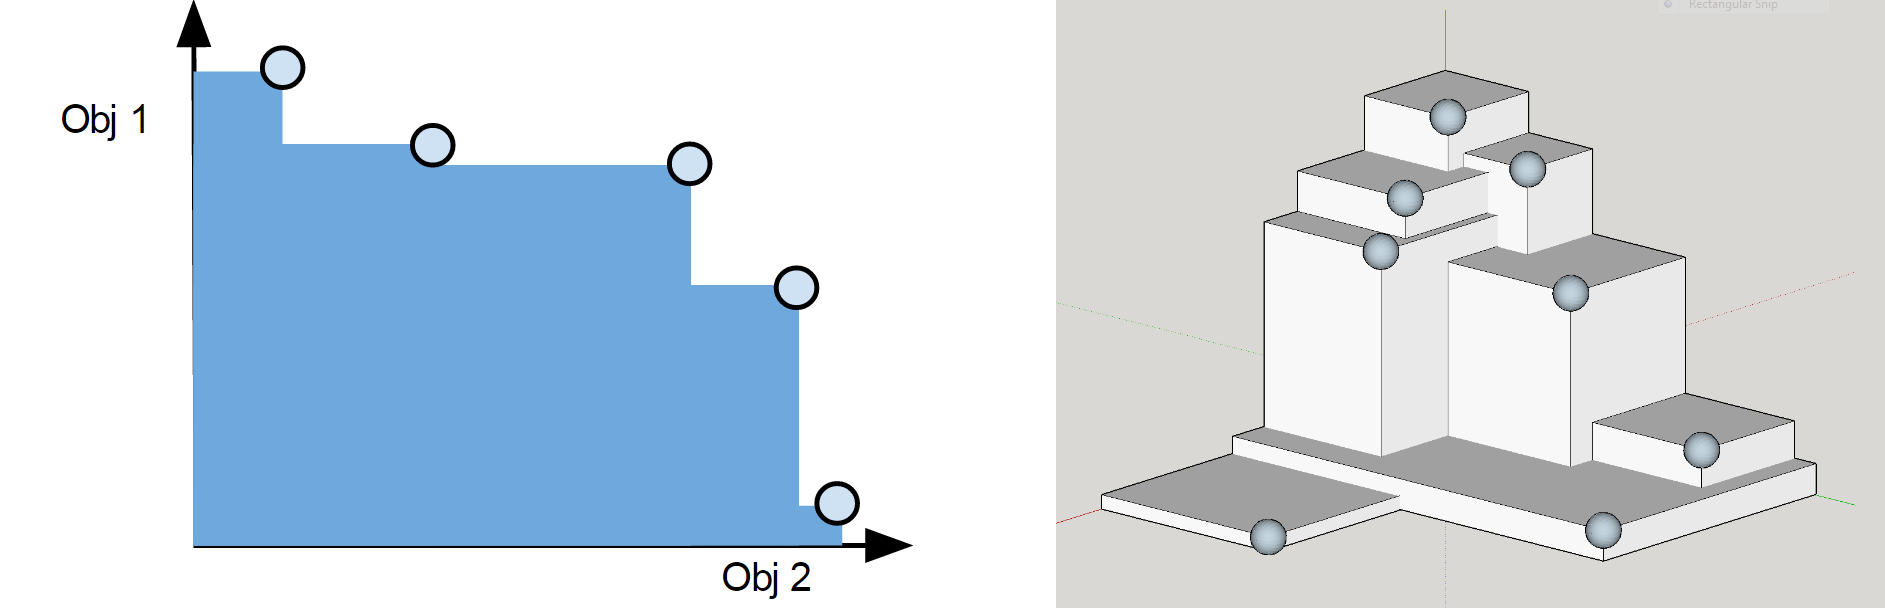
\includegraphics[width=.85\textwidth]{../images/FrontierVolumesConvexNo2DOutlines}
\caption[Hypervolume of Pareto frontiers]{Simple depictions of the hypervolumes of frontiers with two maximization objectives (left) and three maximization objectives (right).}
\label{fig:frontierVolumes}
\end{figure}

To measure the hypervolume indicator, for each relative objective vector $\overbar{\mathbf{z}^i}$ in the frontier $Z$, define its corresponding hyperrectangle $r_i$. $r_i$ is the $M$-orthotope with opposite corners the origin and the point defined by the components of the relative objective vector $\overbar{\mathbf{z}^i}$. Then the hypervolume indicator is the volume of the union of these hyperrectangles:
\begin{align}
I_{H1}(Z) = \text{vol} \left( \bigcup_{i = 1}^{|Z|} r_i \right). \label{eqn:hypervol}
\end{align}
Given two frontiers $Z^1$ and $Z^2$, how do you interpret a difference in their hypervolumes? Consider Figure \ref{fig:Hypervol10percent} which shows the relative objective space for a two-dimensional frontier. The shaded square in the lower left represents an achievement of 10\% in each objective. Since the objective space of the relative objective vectors is bounded by the $1 \times 1$ square, this corresponds to 1\% of the objective space. So if $Z^1$ and $Z^2$ are bi-objective frontiers ($M=2$) and if $I_{H1}(Z^1) - I_{H1}(Z^2) = 0.01$, then the solutions in frontier $Z^1$ bound an area equivalent to an additional 10\% achievement in each objective beyond that bounded by the solutions in $Z^2$. Small differences in the values of the hypervolume represent significant objective gains.

In general, an increase of $h$ in the value of the hypervolume equates to an increase in each objective of $h^{1/M}$. So if $Z^1$ and $Z^2$ were tri-objective ($M=3$) then an improvement of $.01$ in the value of the hypervolume would represent an improvement of about 22\% in each objective.

\begin{figure}
\centering

\includegraphics[width=.5\textwidth]{../images/HypervolumeImprovements}
\caption[Interpreting differences in hypervolumes]{To compute the hypervolume, we use the relative objective vectors for the solutions in a frontier. Thus, the frontier is bounded by the $M$-cube which has a pair of diagonal corners at the origin and $\vec{1}$. Shown here is the 2-cube (a square) representing the space in which we compute the hypervolume for a bi-objective frontier ($M=2$). The space bound by the shaded square in the lower left represents an achievement of 10\% in each objective yet makes up only 1\% of the objective space. Its intent is to show that small differences in hypervolumes are significant: with two objectives, an improvement of 0.01 in the value of the hypervolume represents an additional achievement of 10\% in each objective.}
\label{fig:Hypervol10percent}
\end{figure}

\subsection{Binary Hypervolume Indicator}
If a frontier $Z^2$ is found to have a smaller hypervolume than another $Z^1$, one may wonder whether $Z^2$ is completely enclosed within $Z^1$ or simply bounds a different but smaller region of the relative objective space. We use the binary hypervolume indicator to address this question. The binary hypervolume $I_{H2}(Z^1,Z^2)$ computes the volume of the objective space bounded by $Z^1$ but not by $Z^2$. See Figure \ref{fig:binaryHypervolume}. As such, if $Z^2$ is completely enclosed within $Z^1$, then $I_{H2}(Z^2,Z^1) \le 0$. On the other hand, if $I_{H2}(Z^2,Z^1) > 0$ then $Z^2$ encloses regions of the objective space that $Z^1$ does not.

Following the definition proposed by Zitzler (1999) \cite{zitzler1999evolutionary}, the \textit{binary hypervolume indicator} of two frontiers $Z^1$ and $Z^2$ is \cite{zitzler1999evolutionary}
\begin{align}
I_{H2} (Z^1,Z^2) = I_{H1} (Z^1 + Z^2) - I_{H1} (Z^2)
\end{align}
where $I_{H1} (Z^1 + Z^2)$ is the hypervolume indicator of the frontier that consists of the non-dominated points in $\{Z^1 \cup Z^2\}$. See the lower-left panel in Figure \ref{fig:binaryHypervolume}.

\begin{figure}[ht]
\centering
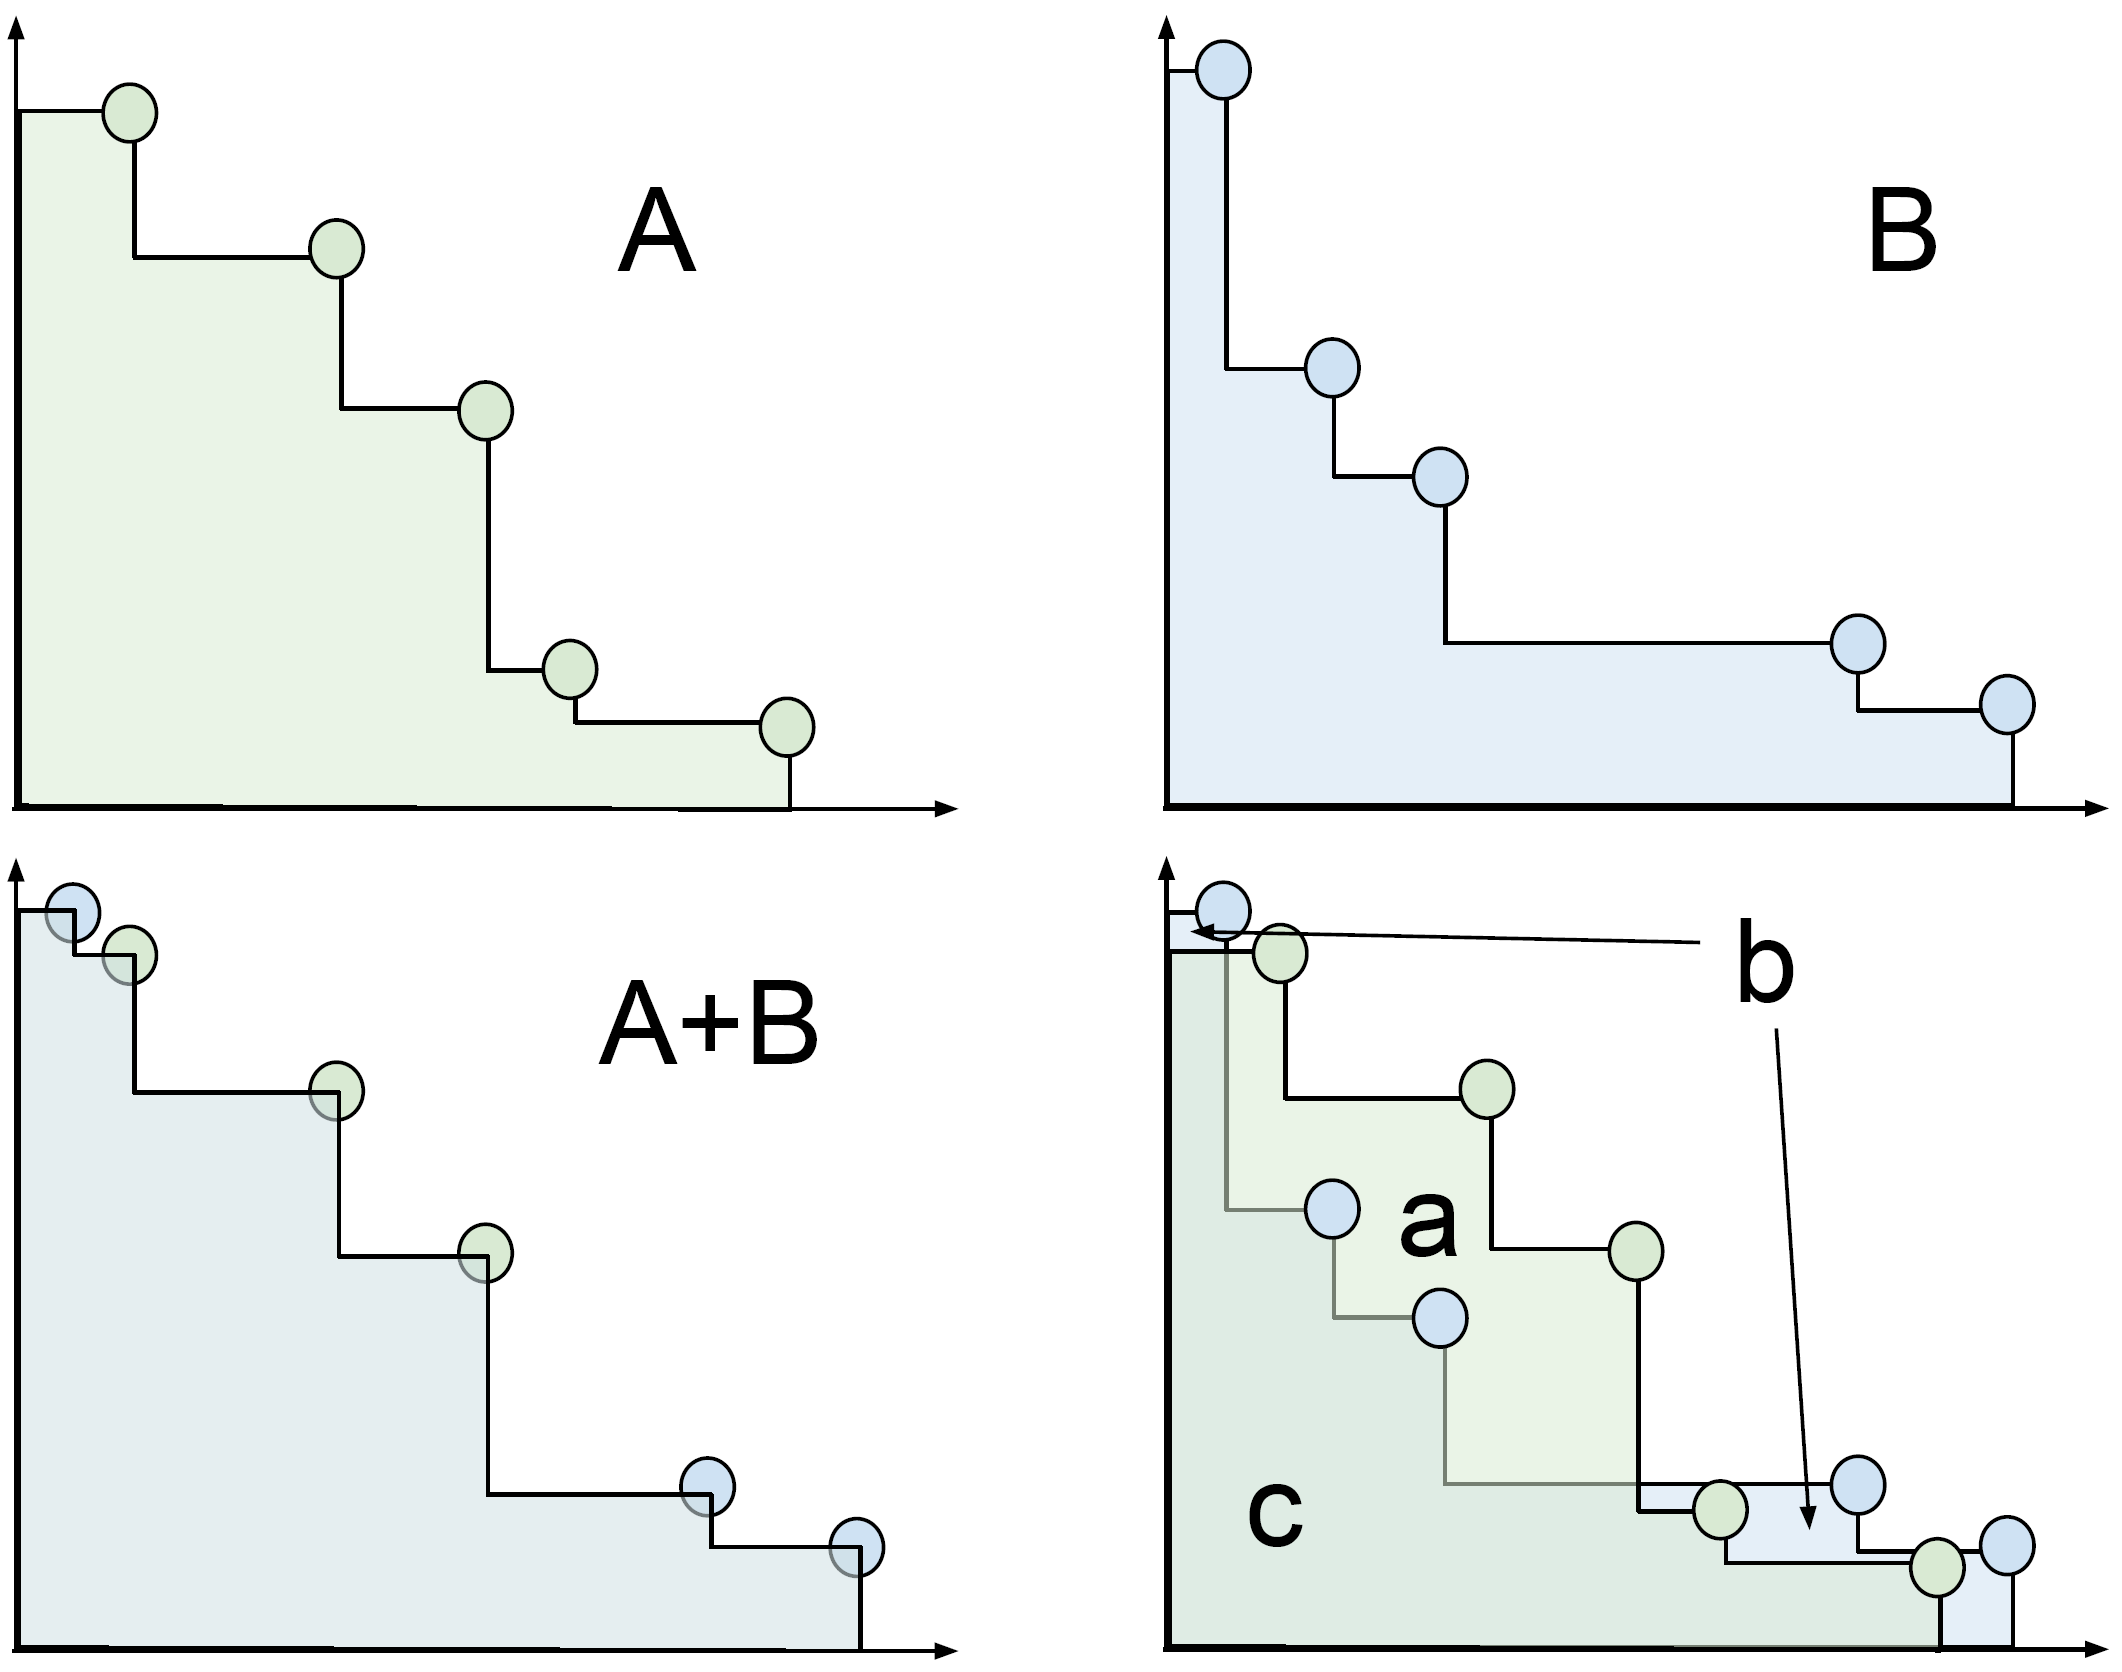
\includegraphics[width=.7\textwidth]{../images/BinaryHypervolume}
\caption[Binary hypervolume indicator]{Depiction of the binary hypervolume indicator. The individual frontiers are shown in the top row: frontier $A$ (left) and frontier $B$ (right). The merged frontier $A+B$ is shown in bottom left - note the absence of points that were dominated when combined. Following the naming of regions as shown in the bottom right figure, the binary hypervolume indicator is equal to
\begin{minipage}{\linewidth}
  \begin{align*}
    I_{H2} (A,B) = \left(\text{area}_a + \text{area}_b + \text{area}_c \right) - \left( \text{area}_b + \text{area}_c \right) = \text{area}_a
  \end{align*}
\end{minipage}%
}
\label{fig:binaryHypervolume}
\end{figure}

\section{Computing the hypervolume indicator}
Computing the hypervolume is a nontrivial task that has received attention from the EMO community. For a comparison of previous algorithms that compute the hypervolume, see While (2006) \cite{while2006faster}. We developed our own algorithm to compute the hypervolume indicator.

The algorithm begins with a list of the relative objective vectors (in describing the algorithm here, we omit the bar and simply denote them by $\mathbf{z} \in Z$). These vectors are assumed to be sorted in descending order based on their $m$th component, for some arbitrary objective $m \in \mathcal{M}$. We define the sub-dimensional objective set $\mathcal{L} = \mathcal{M} \backslash \{m\}$ whose cardinality we denote by $|\mathcal{L}| = L = M - 1$.

We initialize the algorithm with an empty set $G$ of non-dominated solutions in $L$ dimensions. Let the volume of this set be denoted $\overbar{V}$. We add solutions $\mathbf{z}$ from $Z$ to $G$ in order of decreasing $z_m$, at each iteration adding the contribution of the solution $\mathbf{z}$ to the hypervolume indicator $V$. These contributions are computed by multiplying the solution's $m$th component $z_m$ by $\overbar{V}_\mathbf{z}$, its contribution to the volume of $G$. See Figure \ref{fig:AlgoAid} for a visual reference (the solutions' contribution to the volume of $G$, $\overbar{V}_\mathbf{z}$, are the yellow regions in the figure).

We compute $\overbar{V}_\mathbf{z}$ as follows. Initialize $\overbar{V}_\mathbf{z} = 0$, and add $\mathbf{z}$ to the set $G$. Remove from $G$ any solutions that are dominated by $\mathbf{z}$ in $L$ dimensions. Add to $\overbar{V}_\mathbf{z}$ the value of the volume of $\mathbf{z}$ in $L$ dimensions (the union of the yellow and gray areas in Figure \ref{fig:AlgoAid}); this is simply the product of its components $z_\ell$ for $\ell \in \mathcal{L}$. Then subtract from $\overbar{V}_\mathbf{z}$ the volume of $G$ prior to the addition of $\mathbf{z}$ (the union of the gray and white areas in Figure \ref{fig:AlgoAid}). The last step is to compute and add back in the volume of the ``sides'' of $G$ that were subtracted in the previous step (the white areas in Figure \ref{fig:AlgoAid}). This ``sides'' volume is computed by taking the sum over each dimension $\ell \in \mathcal{L}$ of the areas along that dimension enclosed by the existing solutions in $G$. Pseudocode for this algorithm is presented in Figure \ref{algo:HypervolAlgo}.

\newpage
\begin{figure}[H]
\caption[Algorithm to compute the hypervolume indicator of a Pareto frontier]{Algorithm to compute the hypervolume $V$ of a Pareto frontier. Prior to running the algorithm, pick an objective $m$ from the objective set $\mathcal{M}$ and define the sub-dimensional objective set $\mathcal{L} = \mathcal{M} \backslash \{m\}$. Then sort $\mathbf{z} \in Z$ in descending order by their $m$th component. Here, $\mathbf{z} \in Z$ is the set of relative objective vectors. Let $\overbar{V_\mathbf{z}}$ be the ($M-1$)-dimensional volume contribution of the solution $\mathbf{z}$, and let $\mathbf{g} \in G$ be the non-dominated objective vectors in $M-1$ dimensions.}
\label{algo:HypervolAlgo}
\begin{algorithmic}[1]

\State $V \gets 0$
\State $\overbar{V} \gets 0$
\State $G \gets \emptyset$

% Iterate over each solution
\ForAll{$\mathbf{z} \in Z$}

	\State $\overbar{V}_\mathbf{z} \gets \prod_{\ell \in \mathcal{L}} z_\ell - \overbar{V}$
		
	\ForAll{$\mathbf{g} \in G$}
		\If{$\forall \ell \in \mathcal{L} \; g_\ell < z_\ell$}
			\State $G \gets G \backslash \{\mathbf{g}\}$
		\EndIf
	\EndFor
	
	% iterate over subdimensions to "add back the sides"	
	\ForAll{$\ell \in \mathcal{L}$}
	
		\State $G_{\mathbf{z},\ell} := \set{\mathbf{g} \in G : g_\ell > z_\ell}$
		
		\State Sort $\mathbf{g} \in G_{\mathbf{z},\ell}$ in ascending order by $\ell$th component, $g_\ell$
		
		\State $v_i \gets z_\ell$
		\ForAll{$\mathbf{g} \in G_{\mathbf{z},\ell}$}
			\State $v_t \gets g_\ell$
			\State $\delta_\ell := v_t - v_i$
			\State $\overbar{V}_\mathbf{z} \gets \overbar{V}_\mathbf{z} + \delta_\ell \prod_{\lambda \in \mathcal{L} \backslash \{\ell\}} g_\lambda$
			\State $v_i \gets v_t$
		\EndFor
		
	\EndFor
	
	\State $G \gets G \cup \{\mathbf{z}\}$
	\State $\overbar{V} \gets \overbar{V} + \overbar{V}_\mathbf{z}$
	\State $V \gets V + z_m \overbar{V}_\mathbf{z}$
\EndFor


\end{algorithmic}
\end{figure}

\begin{figure}[ht]
\centering
\caption[First three iterations for computing the sub-dimensional hypervolume $\overbar{V}$]{\textbf{Computing the hypervolume of a 3D frontier: first three iterations of the algorithm} (process moves from left to right). Consider a three-dimensional frontier $Z$. We sequentially add solutions to a 2D projection of the frontier, seen here. The solutions are added in order of decreasing value in their third component (height -- not seen here). At each iteration, we compute the contribution in 2D as follows: Add the product of the solution's 2D components (the union of the yellow and gray areas). Then subtract all the previous existing 2D frontier area (the union of the gray and white areas). Then add back the value of the sides (white areas). This yields the value of the yellow area. Multiply this value by the third component of the solution to obtain the solution's contribution to the hypervolume $V$.}
\label{fig:AlgoAid}
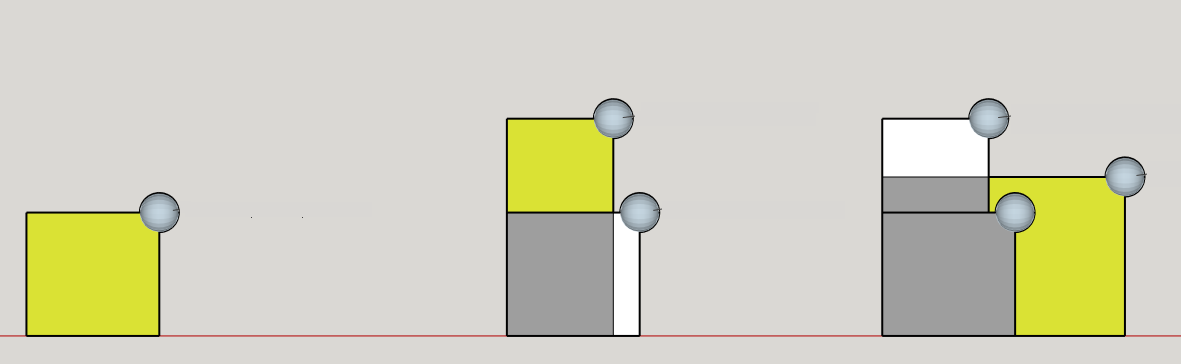
\includegraphics[width=.85\textwidth]{../images/3DFrontierSchematic_SketchUp_FirstSteps_2D_clean}
\end{figure}

\section{A new measure for pairwise objective conflict}
\label{sec:newConflictMetric}
% This is our cool new way of drilling down into an objective pair to assess conflict
When the hypervolume indicates that there is conflict in the system, how does the decision maker determine which objectives are responsible for the conflict? In the case of the hospital, is it cost and patient throughput that are most conflicting, or is it cost and required back-up? For the forest manager, are carbon sequestration and timber revenue the incompatible objectives responsible for the low hypervolume value, or is it wildlife habitat and timber revenue? If the forest manager oversees multiple independent forests, they may also ask whether the answers to these questions are the same in each. With the suite of measures currently available, the decision maker cannot adequately answer these questions. Here we propose a new measure of conflict to fill this void.

To motivate the metric, we consider the simple example in Figure \ref{fig:ConflictVariesExample}. For the frontiers shown here, the conflict between objectives $i$ and $j$ is greatest in Frontier C and least in Frontier A (all objectives are maximized).
\begin{figure}[ht]
\centering

\includegraphics[width=.6\textwidth]{../images/ConflictVariesExample}
\caption[Example of varying conflict between objectives]{Varying conflict between objectives. The conflict between maximization objectives $i$ and $j$ increases from Frontier A to Frontier B to Frontier C.}
\label{fig:ConflictVariesExample}
\end{figure}

Many authors have previously measured conflict between objectives \cite{brockhoff2009objective}\cite{purshouse2003conflict}\cite{gal1977redundant}, with most commonly used metrics deriving from measures of linear correlation (such as the Pearson correlation coefficient \cite{deb2006searching}) or rank correlation (such as Kendall's Tau \cite{kanoulas2009empirical} or Spearman's rho \cite{karande2012application}). The motivation behind these metrics is often the removal of redundant objectives from a many-objective optimization problem. In such cases, these measures of monotonicity or correlation alone suffice. However, they fall short of providing a quantification of conflict between pairs of objectives for the sake of decision making or more general system analysis. For instance, metrics for linear correlation are limited in their ability to capture the montonicity between objectives, which is the fundamental principle that determines if objectives conflict. Furthermore, both linear and rank correlation metrics fail to capture the objective achievement of the solutions. Thus, for a more nuanced understanding of the relationship between the objectives, a different metric is required.

Let $\mathbf{z}_{ij}$ be the sub-dimensional objective vector comprised of only the components corresponding to the $i$th and $j$th objectives $\mathbf{z}_{ij} = [z_i,z_j]$. We define the following measure of conflict between objectives $i$ and $j$:
\begin{align}
C_{ij} = \frac{(1-\rho_{ij})\overbar{d}_{ij}}{2 d_{\max,ij}} \label{eqn:defConflict}
\end{align}
where $\overbar{d}_{ij}$ is the average sub-dimensional distance from objective vectors to the ideal solution:
\begin{align}
\overbar{d}_{ij} = \frac{1}{|Z|} \sum_{\mathbf{z} \in Z} ||\mathbf{z}^{\text{ideal}}_{ij} - \mathbf{z}_{ij}||
\end{align}
and
\begin{align}
d_{\max,ij} = ||\mathbf{z}^{\text{ideal}}_{ij} - \mathbf{z}^{\text{nadir}}_{ij}||
\end{align}
and $\rho_{ij}$ is Spearman's rank-correlation coefficient for the solutions' achievements in objectives $i$ and $j$. Note that $C_{ij} \in [0,1)$, taking smaller values when there is less conflict between objectives $i$ and $j$ and larger values when there is more.

The conflict metric proposed here (equation \eqref{eqn:defConflict}) addresses two major issues:
\begin{enumerate}
\item \textbf{Indifference to non-conflicting relationships}. Per equation \eqref{eqn:objPairHarmony}, when an objective $i$ increases monotonically with another objective $j$, the objectives do not conflict. Accordingly, $C_{ij}$ should equal 0 in all such cases. This is true for the new metric, since for monotonically increasing objectives $\rho_{ij} = 1$, so $1-\rho_{ij} = 0$.
\item \textbf{Consideration of objective achievement}. Recall Figure \ref{fig:ConflictVariesExample} and the intuitive notion that the conflict between objectives $i$ and $j$ is stronger in Frontier C than it is in Frontier B than it is in Frontier A. This notion is guided by the idea that the closer objective vectors are to the sub-dimensional ideal solution on average, the less the conflict between the objectives; that is, that greater simultaneous objective provision is indicative of less conflict. The proposed metric accounts for this, while correlation measures do not. In the extreme case of monotonically decreasing objectives, $\frac{(1-\rho_{ij})}{2} = 1$, so $C_{ij} = \frac{\overbar{d}{ij}}{d_{\max,ij}}$. See Figure \ref{fig:WhyOursIsBetter} for an example.
\end{enumerate}
\begin{figure}[ht]
\centering

\includegraphics[width=.9\textwidth]{../images/WhyOursIsBetter}
\caption[Comparing the proposed conflict metric to others used in multi-objective optimization]{Comparing the proposed metric for conflict $C_{ij}$ against the Pearson product-moment and the Spearman rank correlation coefficients ($\rho_{ij}$ and $\rho_{s,ij}$, respectively). While the latter two are identical for frontiers A and C, the proposed metric is greater for frontier C than it is for A. This is because it accounts for the average relative distance to the sub-dimensional ideal objective vector.}
\label{fig:WhyOursIsBetter}
\end{figure}

To interpret differences in $C_{ij}$ for different objective pairs, we may decompose the metric into components: one for rank correlation
\begin{align}
c_{ij,\rho} = \frac{1-\rho_{ij}}{2},
\end{align}
and one for objective achievement
\begin{align}
c_{ij,d} = \frac{\overbar{d}{ij}}{d_{\max,ij}}.
\end{align}
The comparison of these components for different objective pairs can be used to infer whether the solutions primarily vary in their joint provision of objectives or in their general ordering. For large enough frontiers, a significance test is available for $\rho_{ij}$ to determine whether it is significantly different from 0 (if $c_{ij,\rho}$ is significantly different from 0.5).